% Book 4, Year 2, chapter 27 -- Randomised algorithms.
% Provenance (never printed): sources/book4/BRIEFS.md, chapter 27.
\chapter{Randomised Algorithms}\label{ch:b2:randomised-algorithms}

The town keeps its 120 people in a list sorted by name. A quicksort that takes the first element as its pivot, given
that list again, does the worst thing it can:

\omcode{code/bachelor-2/27-randomised-algorithms/listings/sorted_input.py}{7}{16}{The sorted list of the town's people,
sorted again three ways}\label{lst:b2:randomised-algorithms:hook}

\omoutput{code/bachelor-2/27-randomised-algorithms/outputs/sorted_input.txt}{A fixed pivot on sorted input makes every
possible comparison; a shuffle first, or a random pivot, about one eighth of them.}\label{out:b2:randomised-algorithms:hook}

With the first element as pivot, each call splits off one element and compares it with all the others: $n(n-1)/2$
comparisons, as the Year 1 volume counted. Sorted input is not rare, so a library cannot hope that its users avoid it.
Choosing the pivot at random changes the question: there is no bad input any more, only unlucky coins, and the chapter
shows they are rare. It then uses coins to make hash tables safe against an adversary, to store a set in a few bits per
element, to test whether a 256-bit number is prime, and to find the weakest links of a network.

\begin{recall}
The mathematics Year 2 volume: random variables, expectation and its linearity, $E[X + Y] = E[X] + E[Y]$ even when $X$
and $Y$ are dependent; independent events; the geometric law, whose mean is $1/p$; Markov's inequality, $\Pr[X \geq a]
\leq E[X]/a$ for $X \geq 0$. The Year 1 volume: quicksort and its average cost over random inputs; hash tables with
chaining, and the promise that a good hash function keeps the chains short. The grade 9 volume: pseudo-random numbers,
which a program draws from a seed and can draw again.
\end{recall}

\section{Las Vegas and Monte Carlo}\label{sec:b2:randomised-algorithms:kinds}

\begin{definition}[Randomised algorithm, Las Vegas, Monte Carlo]\label{def:b2:randomised-algorithms:las-vegas}
A \emph{randomised algorithm}\index{randomised algorithm} may draw random numbers as it runs; its running time and its
answer are then random variables, for each input. It is a \emph{Las Vegas algorithm}\index{Las Vegas algorithm} if its
answer is always correct and only its running time is random, and a \emph{Monte Carlo algorithm}\index{Monte Carlo
algorithm} if its running time is bounded but its answer may be wrong with some probability.
\end{definition}

Randomised quicksort is Las Vegas: the list always comes out sorted. A primality test that says ``probably prime'' is
Monte Carlo. The listings draw their numbers from \code{random.Random(seed)}: pseudo-random numbers, the same for the
same seed, which is how every output of this chapter reruns identically. The analyses assume truly random draws.

\begin{definition}[Expected running time]\label{def:b2:randomised-algorithms:expected-time}
The \emph{expected running time}\index{expected running time} of a \omterm{def:b2:randomised-algorithms:las-vegas}{randomised algorithm} on an input $x$ is the
expectation, over its random draws, of its running time on $x$. Its expected running time for size $n$ is the largest of
these over the inputs of size $n$.
\end{definition}

This is not an average-case cost. An average over inputs assumes that inputs follow a law, and an adversary, or a user
with a sorted list, can break it. The \omterm{def:b2:randomised-algorithms:expected-time}{expected running time} holds for every input: the randomness is in the algorithm,
where nobody outside can choose it.

\begin{definition}[One-sided error, amplification]\label{def:b2:randomised-algorithms:amplification}
A \omterm{def:b2:randomised-algorithms:las-vegas}{Monte Carlo algorithm} for a yes-or-no question has \emph{one-sided error}\index{one-sided error} if one of its answers
is always right: for instance ``composite'' is always right and ``prime'' is wrong with probability at most $\varepsilon$.
\emph{Amplification}\index{amplification} runs it $k$ times with independent draws and answers ``prime'' only if every
run does.
\end{definition}

\begin{proposition}[Amplification]\label{prop:b2:randomised-algorithms:amplification}
If each run errs with probability at most $\varepsilon$, independently, the amplified algorithm is wrong with probability
at most $\varepsilon^k$, and costs $k$ times as much.
\end{proposition}

\begin{proof}
It is wrong only if all $k$ runs are wrong, which by independence has probability at most $\varepsilon^k$.
\end{proof}

With $\varepsilon = 1/4$ and $k = 40$, the error is at most $2^{-80}$, far below the chance that the hardware errs during
the run. A \omterm{def:b2:randomised-algorithms:las-vegas}{Monte Carlo algorithm} whose answer can be checked cheaply becomes Las Vegas: run it until the check passes
(\cref{exo:b2:randomised-algorithms:7}).

\section{Randomised quicksort and quickselect}\label{sec:b2:randomised-algorithms:quicksort}

\omcode{code/bachelor-2/27-randomised-algorithms/listings/quicksort.py}{4}{28}{Quicksort with a pivot chosen by a
function, and the Fisher--Yates shuffle}\label{lst:b2:randomised-algorithms:quicksort}

Two ways remove the bad inputs: shuffle the list uniformly first, then use any fixed pivot rule; or choose each pivot
uniformly at random. Both give the same law for the number of comparisons. The shuffle of the listing, due to Fisher
and Yates, produces each of the $n!$ orders with probability $1/n!$ (\cref{exo:b2:randomised-algorithms:11}); the
tempting version that swaps each position with any position is biased (\cref{exo:b2:randomised-algorithms:2}).

\begin{omfigure}
\begin{forest}
for tree={font=\small\ttfamily, l sep=10pt, s sep=14pt, draw, rounded corners=2pt, inner sep=2pt}
[{Bea (9)}
  [{Ada (1)} [Aarav]]
  [{Emil (6)}
    [{Chloe (4)} [{Caio (1)} [Ben]] [{Dev (1)} [Dara]]]
    [Farid]]]
\end{forest}
\par\smallskip{\small One run of randomised quicksort on ten first names, printed by \code{quicksort_trace.py}. Each node
is a pivot, with the number of names compared with it; its left subtree sorts the smaller names, its right subtree the
larger ones. The run makes $9 + 1 + 6 + 4 + 1 + 1 = 22$ comparisons. Two names are compared exactly when one of them is
an ancestor of the other.}
\end{omfigure}

The figure shows the key to the analysis. Number the keys $z_1 < z_2 < \dots < z_n$ in sorted order. Two keys are
compared at most once, when one of them is the pivot, and never again since the pivot is then set aside.

\begin{lemma}[Comparison probability]\label{lem:b2:randomised-algorithms:compared}
In randomised quicksort, for $i < j$, the keys $z_i$ and $z_j$ are compared with probability $2/(j - i + 1)$.
\end{lemma}

\begin{proof}
\Cref{exo:b2:randomised-algorithms:8}: $z_i$ and $z_j$ stay in the same call until the first pivot drawn among $z_i,
\dots, z_j$, and they are compared if and only if that pivot is $z_i$ or $z_j$.
\end{proof}

\begin{theorem}[Randomised quicksort]\label{thm:b2:randomised-algorithms:quicksort}
On every list of $n$ distinct keys, randomised quicksort makes on average exactly $2(n + 1)H_n - 4n$ comparisons, where
$H_n = 1 + 1/2 + \dots + 1/n$. This is about $2n \ln n \approx 1.39\, n \log_2 n$.
\end{theorem}

\begin{proof}
Let $X_{ij}$ be $1$ if $z_i$ and $z_j$ are compared and $0$ otherwise. The number of comparisons is $X = \sum_{i < j}
X_{ij}$, and by linearity and \cref{lem:b2:randomised-algorithms:compared},
\[
E[X] = \sum_{i < j} \frac{2}{j - i + 1} = \sum_{k = 2}^{n} (n - k + 1) \frac{2}{k},
\]
grouping the pairs by $k = j - i + 1$, of which there are $n - k + 1$. This is $2(n + 1)\sum_{k = 2}^{n} \frac{1}{k} -
2(n - 1) = 2(n + 1)(H_n - 1) - 2n + 2 = 2(n + 1)H_n - 4n$. Finally $H_n = \ln n + O(1)$.
\end{proof}

\omoutput{code/bachelor-2/27-randomised-algorithms/outputs/quicksort_rand.txt}{1,000 runs on the sorted list of the
town's people, against the exact expectation.}\label{out:b2:randomised-algorithms:quicksort}

The proof uses no independence between the $X_{ij}$, which are far from independent: linearity of expectation is the
whole tool. The output shows more than the mean: in 1,000 runs, none passed one and a half times it, and the largest is
a sixth of the worst case. Bounding the spread needs more than linearity; the chapter keeps to expectations.

The same idea finds the key of a given rank without sorting: partition around a random pivot, and continue only on the
side that contains the rank.

\omcode{code/bachelor-2/27-randomised-algorithms/listings/quickselect.py}{7}{19}{Quickselect: the key of rank $k$ with
a random pivot}\label{lst:b2:randomised-algorithms:quickselect}

\begin{theorem}[Quickselect]\label{thm:b2:randomised-algorithms:quickselect}
On every list of $n$ distinct keys and every rank, quickselect makes on average at most $4n$ comparisons.
\end{theorem}

\begin{proof}
Let $T(n)$ be the largest expected number of comparisons over lists of size $n$ and ranks. The partition costs $n - 1$;
the pivot has rank $i$ with probability $1/n$, for $0 \leq i \leq n - 1$, and the search continues on a side of size at
most $\max(i, n - 1 - i)$. So $T(n) \leq n - 1 + \frac{1}{n} \sum_{i = 0}^{n - 1} T(\max(i, n - 1 - i))$, and $T(0) =
T(1) = 0$. Assume $T(k) \leq 4k$ for $k < n$. The values $\max(i, n - 1 - i)$ run through the upper half of $0, \dots, n
- 1$ twice, and their sum is at most $3n^2/4$ (check $n = 2r$ and $n = 2r + 1$). Then $T(n) \leq n - 1 + \frac{4}{n}
\cdot \frac{3n^2}{4} = 4n - 1$.
\end{proof}

\omoutput{code/bachelor-2/27-randomised-algorithms/outputs/quickselect.txt}{The smallest, the median and the largest name,
1,000 runs each.}\label{out:b2:randomised-algorithms:quickselect}

The median is the most expensive rank, about $3.1\,n$ here; the exact expectation for the median is close to
$2(1 + \ln 2) n \approx 3.39\, n$ for large $n$, and $4n$ is a simple bound above it.

\begin{history}
% ledger: b2:hoare-1961
Tony Hoare published Quicksort in 1961, as an algorithm of a few lines in the journal of the computing society of the
time.
\end{history}

\section{Universal hashing}\label{sec:b2:randomised-algorithms:universal}

A hash table with a fixed function such as $h(x) = x \bmod m$ has bad inputs too: keys that are all multiples of $m$ all
land in bucket $0$. If the keys come from outside, from names typed in a form or from packets on a network, someone can
send exactly those, and every lookup becomes a walk along a list of all the keys. The cure is the same as for quicksort:
choose the function at random, after the keys are fixed.

\begin{definition}[Universal family]\label{def:b2:randomised-algorithms:universal}
A set $\mathcal{H}$ of functions from the keys to $\{0, \dots, m - 1\}$ is a \emph{universal family}\index{universal
family of hash functions} if for any two distinct keys $x \neq y$, a function $h$ drawn uniformly from $\mathcal{H}$
makes them collide with probability at most $1/m$: $\Pr[h(x) = h(y)] \leq 1/m$.
\end{definition}

\begin{theorem}[Carter--Wegman]\label{thm:b2:randomised-algorithms:carter-wegman}
Let $p$ be a prime larger than every key and $m \geq 2$. The functions $h_{a,b}(x) = ((ax + b) \bmod p) \bmod m$, for
$1 \leq a \leq p - 1$ and $0 \leq b \leq p - 1$, form a \omterm{def:b2:randomised-algorithms:universal}{universal family}.
\end{theorem}

\begin{proof}
Fix keys $x \neq y$ in $\{0, \dots, p - 1\}$, and let $r = (ax + b) \bmod p$, $s = (ay + b) \bmod p$. Then $r - s \equiv
a(x - y) \pmod p$, and since $p$ is prime and neither $a$ nor $x - y$ is a multiple of $p$, $r \neq s$. Conversely, given
$r \neq s$, the equations determine $a = (r - s)(x - y)^{-1} \bmod p$, which is not $0$, and then $b = (r - ax) \bmod p$:
the map $(a, b) \mapsto (r, s)$ is a bijection from the $p(p - 1)$ functions onto the pairs $r \neq s$. Drawing $(a, b)$
uniformly therefore draws $(r, s)$ uniformly among the pairs of distinct values. The keys collide when $r \equiv s
\pmod m$. For each $r$, the values $s \neq r$ in $\{0, \dots, p - 1\}$ with $s \equiv r \pmod m$ number at most $\lceil p/m
\rceil - 1 \leq (p - 1)/m$. So the colliding pairs number at most $p(p - 1)/m$, out of $p(p - 1)$.
\end{proof}

The modular inverse used in the proof exists because $p$ is prime, the property the mathematics books prove with
B\'ezout's identity; the program never computes it.

\begin{corollary}[Short chains]\label{cor:b2:randomised-algorithms:chains}
Store $n$ keys in a table of $m$ buckets with chaining, with a function drawn from a \omterm{def:b2:randomised-algorithms:universal}{universal family}. For every key $x$
of the table, the expected length of its chain is at most $1 + (n - 1)/m < 1 + \alpha$, where $\alpha = n/m$. For a key
not in the table, the expected length of the chain it lands in is at most $\alpha$.
\end{corollary}

\begin{proof}
The chain of $x$ holds $x$ and the keys $y \neq x$ with $h(y) = h(x)$. Its length is $1 + \sum_{y \neq x} C_y$, where
$C_y$ is $1$ on a collision, and $E[C_y] \leq 1/m$. By linearity, the expectation is at most $1 + (n - 1)/m$. For a key
not in the table, the same sum has $n$ terms and no $1$.
\end{proof}

This is the promise the Year 1 volume made for hash tables, now kept for every set of keys, with the randomness in the
choice of the function. The listing attacks both kinds of function with keys that are all multiples of $m$.

\omcode{code/bachelor-2/27-randomised-algorithms/listings/universal_hash.py}{5}{18}{A function drawn from the
Carter--Wegman family, and the chain lengths it gives}\label{lst:b2:randomised-algorithms:universal}

\omoutput{code/bachelor-2/27-randomised-algorithms/outputs/universal_hash.txt}{Keys that are all multiples of $m$: one
chain of $n$ keys for $x \bmod m$; for a random member of the family, the median longest chain over 1,000 draws, and the
average chain length seen by a key, against the bound.}\label{out:b2:randomised-algorithms:universal}

\begin{omfigure}
\begin{tikzpicture}
\begin{axis}[width=0.72\linewidth, height=5.2cm, ymode=log, xlabel={number of keys $n$ (with $m = n$ buckets)},
  ylabel={longest chain}, legend style={font=\small, at={(0.97,0.5)}, anchor=east}, grid=major, xtick={200,400,600,800,1000},
  ymin=1, ymax=3000]
  \addplot[omDef, thick, mark=*, mark size=1.5pt] table[x=n, y=fixed]
    {code/bachelor-2/27-randomised-algorithms/figures/chains.dat};
  \addlegendentry{$h(x) = x \bmod m$}
  \addplot[omThm, thick, mark=square*, mark size=1.5pt] table[x=n, y=universal]
    {code/bachelor-2/27-randomised-algorithms/figures/chains.dat};
  \addlegendentry{drawn from the family (median)}
\end{axis}
\end{tikzpicture}
\par\smallskip{\small The longest chain under the attack of \cref{out:b2:randomised-algorithms:universal}, on a
logarithmic scale: all $n$ keys in one chain for the fixed function, five for a function drawn after the keys.}
\end{omfigure}

The measured average chain of a key matches the bound $1 + (n - 1)/m$ to within the noise of 1,000 draws: for these
keys the bound is reached. The adversary has not disappeared: once a function is drawn, keys exist that collide under
it. A server must therefore keep its draw secret, and libraries of several languages draw a secret seed for their
string hashing when the program starts.

\begin{history}
% ledger: b2:carter-wegman-1979
Lawrence Carter and Mark Wegman defined universal classes of hash functions in 1979, with the family of
\cref{thm:b2:randomised-algorithms:carter-wegman} among their examples.
\end{history}

\section{Bloom filters}\label{sec:b2:randomised-algorithms:bloom}

A set of a million long strings takes megabytes as a hash table. Often one only needs to answer ``certainly not in the
set'' quickly, and to look further for the rest: a browser checking addresses against a list of known bad sites, a
database checking whether a disk block might hold a key before reading it.

\begin{definition}[Bloom filter, false positive]\label{def:b2:randomised-algorithms:bloom}
A \emph{Bloom filter}\index{Bloom filter} is an array of $m$ bits, all $0$ at first, and $k$ hash functions $h_1, \dots,
h_k$ with values in $\{0, \dots, m - 1\}$. Adding a key $x$ sets the bits $h_1(x), \dots, h_k(x)$ to $1$. A lookup of
$y$ answers ``present'' if its $k$ bits are all $1$. A \emph{false positive}\index{false positive (Bloom filter)} is a
lookup that answers ``present'' for a key that was never added.
\end{definition}

A key that was added always finds its bits set: there are no false negatives. Keys cannot be removed, since a bit may be
shared.

\omcode{code/bachelor-2/27-randomised-algorithms/listings/bloom.py}{9}{19}{A \omterm{def:b2:randomised-algorithms:bloom}{Bloom filter} whose $k$ functions are drawn
independently from the \omterm{def:b2:randomised-algorithms:universal}{universal family}}\label{lst:b2:randomised-algorithms:bloom}

\omoutput{code/bachelor-2/27-randomised-algorithms/outputs/bloom_small.txt}{Three names in 16 bits with 3 functions, and
the other first names of the town looked up.}\label{out:b2:randomised-algorithms:bloom-small}

\begin{omfigure}
\begin{tikzpicture}[x=6.5mm, y=6.5mm, bit/.style={draw, minimum size=6.5mm, inner sep=0pt, font=\small\ttfamily},
  arr/.style={->, >=Stealth, thin}]
\foreach \b [count=\i from 0] in {0,0,0,0,0,1,1,0,1,1,1,1,0,0,0,1} {
  \ifnum\b=1 \node[bit, fill=omDef!25] (b\i) at (\i, 0) {1};
  \else \node[bit] (b\i) at (\i, 0) {0}; \fi
  \node[font=\tiny, above, inner sep=1pt] (l\i) at (\i, 0.33) {\i};
}
\node[font=\small] (ada) at (3, 3.2) {Ada};
\node[font=\small] (ben) at (8, 3.2) {Ben};
\node[font=\small] (cy) at (12.5, 3.2) {Cy};
\foreach \t in {15, 5, 11} \draw[arr, omDef] (ada) -- (l\t.north);
\foreach \t in {8, 10, 6} \draw[arr, omThm] (ben) -- (l\t.north);
\foreach \t in {9, 6, 11} \draw[arr, black!60] (cy) -- (l\t.north);
\node[font=\small] (hana) at (8.5, -2.9) {Hana: present?};
\foreach \t in {10, 11, 6} \draw[arr, red!70!black, dashed] (hana) -- (b\t.south);
\end{tikzpicture}
\par\smallskip{\small The filter of \cref{out:b2:randomised-algorithms:bloom-small}. Each added name sets 3 bits; the
bits 6 and 11 are shared. Hana was never added, but her bits 10, 11 and 6 were all set by Ben and Cy: a \omterm{def:b2:randomised-algorithms:bloom}{false positive}.}
\end{omfigure}

\begin{proposition}[False-positive rate]\label{prop:b2:randomised-algorithms:bloom-rate}
Assume that the $kn$ hash values of $n$ added keys, and the $k$ values of a key looked up, are independent and uniform on
$\{0, \dots, m - 1\}$. After $n$ keys, a given bit is still $0$ with probability $(1 - 1/m)^{kn} \approx e^{-kn/m}$, and
if the bits are treated as independent, a key not added is a \omterm{def:b2:randomised-algorithms:bloom}{false positive} with probability about
\[
\left(1 - e^{-kn/m}\right)^k .
\]
For a given ratio $m/n$ this is smallest for $k = (m/n) \ln 2$, where it is $2^{-k} \approx 0.6185^{m/n}$.
\end{proposition}

\begin{proof}
Each of the $kn$ values misses a given bit with probability $1 - 1/m$, independently; and $(1 - 1/m)^{kn} = e^{kn \ln(1 -
1/m)} \approx e^{-kn/m}$ for large $m$. A key not added is a \omterm{def:b2:randomised-algorithms:bloom}{false positive} when its $k$ bits are $1$; treating them as
independent gives the formula. Write $q = e^{-kn/m}$, so that $k = -(m/n) \ln q$ and the logarithm of the rate is $k \ln(1
- q) = -(m/n) \ln q \ln(1 - q)$. The product $\ln q \ln(1 - q)$ is symmetric in $q$ and $1 - q$, and largest at $q =
1/2$, which minimises the rate: then $k = (m/n) \ln 2$ and the rate is $(1/2)^k = 2^{-(m/n)\ln 2} \approx 0.6185^{m/n}$.
\end{proof}

The independence of the bits is an approximation; the measurement shows it is a good one. With 8 bits per key the best
rate is about $2\%$, with 10 bits about $0.8\%$, whatever the length of the keys.

\omoutput{code/bachelor-2/27-randomised-algorithms/outputs/bloom.txt}{1,000 keys in 8,000 bits, measured with 100,000
other keys for each $k$.}\label{out:b2:randomised-algorithms:bloom}

\begin{omfigure}
\begin{tikzpicture}
\begin{axis}[width=0.72\linewidth, height=5.2cm, xlabel={number of hash functions $k$}, ylabel={false-positive rate},
  legend pos=north east, legend style={font=\small}, grid=major, xtick={1,...,10}, ymin=0, ymax=0.13,
  yticklabel style={/pgf/number format/fixed}]
  \addplot[omThm, thick, domain=1:10, samples=91] {(1 - exp(-x/8))^x};
  \addlegendentry{$(1 - e^{-kn/m})^k$}
  \addplot[omDef, only marks, mark=*, mark size=2pt] table[x=k, y=measured]
    {code/bachelor-2/27-randomised-algorithms/figures/bloom.dat};
  \addlegendentry{measured}
\end{axis}
\end{tikzpicture}
\par\smallskip{\small The false-positive rate of \cref{out:b2:randomised-algorithms:bloom} against the formula of
\cref{prop:b2:randomised-algorithms:bloom-rate}, for $m/n = 8$. Too few functions leave each lookup a weak test; too many
fill the array with ones. The minimum is near $k = 8 \ln 2 \approx 5.5$.}
\end{omfigure}

\begin{inpractice}
% ledger: b2:bloom-1970
Burton Bloom described the structure in 1970, for a dictionary too large for memory. Storage engines that keep sorted
files of keys on disk put a \omterm{def:b2:randomised-algorithms:bloom}{Bloom filter} in front of each file, so that most lookups of absent keys never read the file.
\end{inpractice}

\section{Primality}\label{sec:b2:randomised-algorithms:primality}

Public-key cryptography needs random primes of hundreds of bits. Trial division up to $\sqrt{n}$ takes about $2^{128}$
steps for a 256-bit number. A randomised test takes a few modular exponentiations, each $O(\log n)$ multiplications by
repeated squaring.

\begin{definition}[Fermat witness, Carmichael number]\label{def:b2:randomised-algorithms:fermat}
Let $n > 2$ be odd and $1 \leq a \leq n - 1$. If $a^{n-1} \not\equiv 1 \pmod n$, then $a$ is a \emph{Fermat
witness}\index{Fermat witness} for $n$; otherwise $n$ \emph{passes} for the base $a$. A \emph{Carmichael
number}\index{Carmichael number} is an odd composite number that passes for every base coprime to it.
\end{definition}

\begin{proposition}[The Fermat test]\label{prop:b2:randomised-algorithms:fermat}
If $n$ is prime, it passes for every base. If $n$ is composite and has at least one \omterm{def:b2:randomised-algorithms:fermat}{Fermat witness} coprime to it, then at
least half of the bases coprime to $n$ are Fermat witnesses.
\end{proposition}

\begin{proof}
The first part is Fermat's little theorem, from the mathematics books. For the second, let $a$ be a witness coprime to
$n$ and $b_1, \dots, b_r$ the bases coprime to $n$ for which $n$ passes. The products $ab_i \bmod n$ are coprime to $n$
and distinct, since $a$ is invertible modulo $n$. Each is a witness: $(ab_i)^{n-1} = a^{n-1} b_i^{n-1} \equiv a^{n-1}
\not\equiv 1$. So there are at least as many witnesses as passing bases.
\end{proof}

The \omterm{def:b2:randomised-algorithms:fermat}{Carmichael numbers} escape the second part, and they exist: $561 = 3 \cdot 11 \cdot 17$ is the smallest. A sharper
test asks more of a prime.

\begin{definition}[Miller--Rabin witness]\label{def:b2:randomised-algorithms:miller-rabin}
Let $n > 2$ be odd, and write $n - 1 = 2^s d$ with $d$ odd. A base $a$ is a \emph{Miller--Rabin witness}\index{Miller--Rabin
witness} for $n$ if $a^d \not\equiv 1$ and $a^{2^i d} \not\equiv -1 \pmod n$ for every $0 \leq i < s$.
\end{definition}

A prime $p$ has no \omterm{def:b2:randomised-algorithms:miller-rabin}{Miller--Rabin witness}. The sequence $a^d, a^{2d}, \dots, a^{2^s d} = a^{p-1}$ ends with $1$, by
Fermat, and each term is the square of the one before. If $x^2 \equiv 1 \pmod p$, then $p$ divides $(x - 1)(x + 1)$, so
$x \equiv \pm 1$: the term before the first $1$, if there is one, is $-1$.

\omcode{code/bachelor-2/27-randomised-algorithms/listings/primality.py}{9}{32}{The Miller--Rabin test for one base, and
the amplified Monte Carlo test}\label{lst:b2:randomised-algorithms:primality}

\begin{theorem}[Miller--Rabin]\label{thm:b2:randomised-algorithms:miller-rabin}
If $n > 4$ is odd and composite, at most a quarter of the bases $1 \leq a \leq n - 1$ are not Miller--Rabin witnesses.
So $k$ rounds with independent uniform bases answer ``prime'' for a composite number with probability at most $4^{-k}$.
\end{theorem}

\admitted

The proof uses the structure of the group of units modulo $n$ and the Chinese remainder theorem, which the mathematics
books develop. The second sentence follows by \cref{prop:b2:randomised-algorithms:amplification}.

\omoutput{code/bachelor-2/27-randomised-algorithms/outputs/fermat_mr.txt}{Three \omterm{def:b2:randomised-algorithms:fermat}{Carmichael numbers} and a prime, every base
tried.}\label{out:b2:randomised-algorithms:fermat}

The three \omterm{def:b2:randomised-algorithms:fermat}{Carmichael numbers} pass the Fermat test for all their coprime bases, and the Miller--Rabin test catches them
with more than $90\%$ of the bases. To draw a random prime of 256 bits, draw random odd numbers of 256 bits until one
passes. By the prime number theorem, a number near $N$ is prime with probability about $1/\ln N$, an odd one about
$2/\ln N$; the number of draws follows a geometric law of mean about $\ln N / 2$.

\omoutput{code/bachelor-2/27-randomised-algorithms/outputs/random_prime.txt}{200 random primes of 256 bits: the number of
odd numbers tried for each.}\label{out:b2:randomised-algorithms:random-prime}

The mean is close to $\ln(2^{256})/2$; the largest, 512, shows how long the tail of a geometric law is. The candidates
are close to $2^{255}$ and $2^{256}$, where primes are a little rarer than $1/\ln 2^{255}$ suggests, which explains part of
the difference.

\begin{history}
% ledger: b2:miller-1976
% ledger: b2:rabin-1980
Gary Miller published in 1976 a test that is correct if a form of the Riemann hypothesis holds; Michael Rabin made it
probabilistic, with a proven error bound and no hypothesis, in a paper published in 1980.
\end{history}

\section{Random choices that approximate}\label{sec:b2:randomised-algorithms:approximate}

\paragraph{Satisfying many clauses.} Some problems are hard to solve exactly but easy to solve well by tossing coins. In
the satisfiability problem of \cref{ch:b2:predicate-logic}, a formula is a conjunction of clauses, and one may ask for an
assignment that satisfies as many clauses as possible.

\begin{proposition}[A random assignment]\label{prop:b2:randomised-algorithms:maxsat}
Give each variable the value true or false with probability $1/2$, independently. A clause of $k$ literals on distinct
variables is satisfied with probability $1 - 2^{-k}$. So the expected number of satisfied clauses is at least half of
them, and at least three quarters if every clause has two literals or more.
\end{proposition}

\begin{proof}
The clause is false only if each of its $k$ literals is false, which happens with probability $2^{-k}$ since the
variables are distinct and independent. Summing over the clauses with linearity gives the expected number, and $1 -
2^{-k} \geq 1/2$, or $\geq 3/4$ when $k \geq 2$.
\end{proof}

\omoutput{code/bachelor-2/27-randomised-algorithms/outputs/maxsat.txt}{Random assignments on 200 clauses of two literals,
then on a mix of one, two and three.}\label{out:b2:randomised-algorithms:maxsat}

An expectation is reached by some outcome: an assignment satisfying at least three quarters of the 2-literal clauses
always exists, which the proposition proves without exhibiting one.

\paragraph{Karger's minimum cut.} A \emph{cut} of an undirected graph splits its vertices into two non-empty parts; its
size is the number of edges between them. Unlike the cuts of \cref{ch:b2:flows-and-matchings}, no source or sink is
fixed: the question is the smallest cut of all.

\begin{definition}[Edge contraction]\label{def:b2:randomised-algorithms:contraction}
In a multigraph (a graph that may have several edges between two vertices), \emph{contracting}\index{edge contraction}
an edge $\{u, v\}$ replaces $u$ and $v$ by a single vertex, keeps every other edge of $u$ or $v$ with its end moved to the
new vertex, and removes the edges between $u$ and $v$, which would become loops.
\end{definition}

Karger's algorithm contracts a uniformly random edge until two vertices remain, and returns the edges between them. Each
vertex then stands for a set of original vertices, and the edges between the two are a cut of the original graph.

\omcode{code/bachelor-2/27-randomised-algorithms/listings/karger.py}{11}{35}{Karger's algorithm: the contractions as
unions, the edges taken in a random order}\label{lst:b2:randomised-algorithms:karger}

The listing does not build the multigraph. It takes the edges in a random order and contracts each one unless its ends
are already merged. An edge whose ends are merged is exactly a loop, so the first edge of the order that is not a loop is
uniform among the edges that remain: the same law as the algorithm.

\omoutput{code/bachelor-2/27-randomised-algorithms/outputs/karger_demo.txt}{Two groups of four friends joined by two
friendships: one run, and the success rate.}\label{out:b2:randomised-algorithms:karger}

\begin{omfigure}
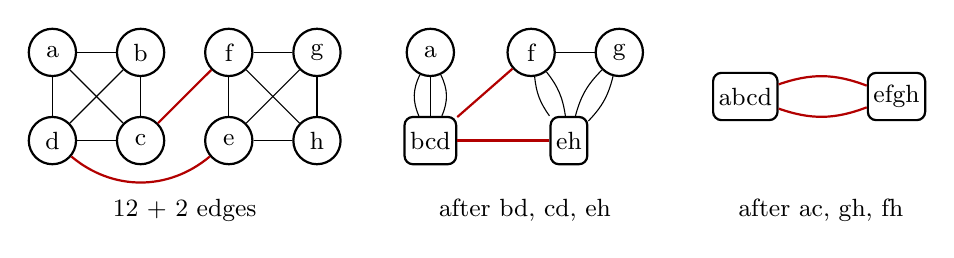
\begin{tikzpicture}[v/.style={circle, draw, thick, minimum size=6mm, inner sep=0pt, font=\small},
  s/.style={rounded corners=3pt, draw, thick, minimum height=6mm, inner sep=2pt, font=\small}, x=8mm, y=8mm]
\begin{scope}
\node[v] (a) at (0, 1) {a}; \node[v] (b) at (1.4, 1) {b};
\node[v] (c) at (1.4, -0.4) {c}; \node[v] (d) at (0, -0.4) {d};
\node[v] (e) at (2.8, -0.4) {e}; \node[v] (f) at (2.8, 1) {f};
\node[v] (g) at (4.2, 1) {g}; \node[v] (h) at (4.2, -0.4) {h};
\foreach \u/\w in {a/b, a/c, a/d, b/c, b/d, c/d, e/f, e/g, e/h, f/g, f/h, g/h} \draw (\u) -- (\w);
\draw[red!70!black, thick] (d) to[bend right=40] (e);
\draw[red!70!black, thick] (c) -- (f);
\node[font=\small] at (2.1, -1.5) {12 + 2 edges};
\end{scope}
\begin{scope}[xshift=48mm]
\node[v] (a) at (0, 1) {a}; \node[s] (B) at (0, -0.4) {bcd};
\node[s] (E) at (2.2, -0.4) {eh}; \node[v] (f) at (1.6, 1) {f}; \node[v] (g) at (3, 1) {g};
\draw (a) to[bend left=25] (B); \draw (a) -- (B); \draw (a) to[bend right=25] (B);
\draw[red!70!black, thick] (B) -- (E); \draw[red!70!black, thick] (B) -- (f);
\draw (E) to[bend left=15] (f); \draw (E) to[bend right=15] (f);
\draw (E) to[bend left=15] (g); \draw (E) to[bend right=15] (g); \draw (f) -- (g);
\node[font=\small] at (1.5, -1.5) {after bd, cd, eh};
\end{scope}
\begin{scope}[xshift=88mm]
\node[s] (L) at (0, 0.3) {abcd}; \node[s] (R) at (2.4, 0.3) {efgh};
\draw[red!70!black, thick] (L) to[bend left=20] (R); \draw[red!70!black, thick] (L) to[bend right=20] (R);
\node[font=\small] at (1.2, -1.5) {after ac, gh, fh};
\end{scope}
\end{tikzpicture}
\par\smallskip{\small The run of \cref{out:b2:randomised-algorithms:karger}. The three contractions $bd$, $cd$, $eh$
leave five vertices and a multigraph (three edges between $a$ and $bcd$); three more leave two, joined by the two red
edges, the minimum cut. A run fails as soon as it contracts a red edge.}
\end{omfigure}

\begin{theorem}[Karger]\label{thm:b2:randomised-algorithms:karger}
Let $C$ be a minimum cut of a connected multigraph with $n \geq 2$ vertices. One run of the contraction algorithm returns
exactly $C$ with probability at least $2/(n(n - 1))$. With $\frac{n(n - 1)}{2} \ln \frac{1}{\delta}$ independent runs,
keeping the smallest cut found, it misses every minimum cut with probability at most $\delta$.
\end{theorem}

\begin{proof}
Let $c = |C|$. The run returns $C$ if it never contracts an edge of $C$: then the two final vertices are the two sides of
$C$. Every vertex of the multigraph has degree at least $c$ at every stage, since the edges at a vertex form a cut of the
original graph (its set of original vertices against the rest). With $r$ vertices left there are therefore at least $rc/2$
edges, and a uniform edge is in $C$ with probability at most $c/(rc/2) = 2/r$, if no edge of $C$ was contracted yet. The
stages have $r = n, n - 1, \dots, 3$ vertices, so the run avoids $C$ with probability at least
\[
\prod_{r = 3}^{n} \left(1 - \frac{2}{r}\right) = \prod_{r = 3}^{n} \frac{r - 2}{r} = \frac{1 \cdot 2}{(n - 1) n},
\]
the product telescoping. With $N$ independent runs, all of them miss $C$ with probability at most $(1 - 2/(n(n -
1)))^N \leq e^{-2N/(n(n - 1))}$, using $1 - x \leq e^{-x}$; this is $\delta$ for the $N$ of the statement.
\end{proof}

The bound is for one given minimum cut, in the worst graph. The measured success in
\cref{out:b2:randomised-algorithms:karger}, about $21\%$, is six times the bound $3.6\%$. A run is a near-linear pass over
the edges, and $O(n^2 \log n)$ runs give a total far above the cost of the best methods, but the algorithm is three lines
and its analysis one product.

\begin{history}
% ledger: b2:karger-1993
David Karger published the contraction algorithm in 1993.
\end{history}

\section{Exercises}\label{sec:b2:randomised-algorithms:exercises}

\begin{exercise}[$\star$]\label{exo:b2:randomised-algorithms:1}
$1729 = 7 \cdot 13 \cdot 19$ passes the Miller--Rabin test for 160 of the 1,726 bases from $2$ to $1727$
(\cref{out:b2:randomised-algorithms:fermat}). What does the $k$-round test of \cref{lst:b2:randomised-algorithms:primality}
answer for 1729, and with which probabilities, for $k = 1, 2, 3, 5$? Compare with \code{exo_monte_carlo.py}.
\end{exercise}

\begin{exercise}[$\star$]\label{exo:b2:randomised-algorithms:2}
A shuffle swaps each position $i$ with a position drawn uniformly among all $n$. For $n = 3$, count the $3^3$ sequences of
choices that produce each order, and explain from the numbers $27$ and $6$ why no such shuffle can be uniform. Check with
\code{exo_shuffle.py}.
\end{exercise}

\begin{exercise}[$\star$]\label{exo:b2:randomised-algorithms:3}
Write a function that reads a stream of unknown length once and returns $k$ of its items, each set of $k$ items being
equally likely, keeping only $k$ items in memory. Check it exhaustively for $n = 6$ and $k = 2$.
\end{exercise}

\begin{exercise}[$\star$]\label{exo:b2:randomised-algorithms:4}
A trial succeeds with probability $p$, independently of the others. Prove that the expected number of trials up to the
first success is $1/p$. Deduce the expected number of odd 256-bit numbers drawn in \cref{out:b2:randomised-algorithms:random-prime},
taking the probability that one is prime to be $2/\ln 2^{256}$.
\end{exercise}

\begin{exercise}[$\star\star$]\label{exo:b2:randomised-algorithms:5}
$341 = 11 \cdot 31$. Show that $2^{340} \equiv 1 \pmod{341}$ ($2^{10} = 1024 = 3 \cdot 341 + 1$), so that base 2 does not
reveal 341, but base 3 does. Count the bases that do not reveal it, and show that Miller--Rabin with base 2 does. Check
with \code{exo_341.py}.
\end{exercise}

\begin{exercise}[$\star\star$]\label{exo:b2:randomised-algorithms:6}
A \omterm{def:b2:randomised-algorithms:bloom}{Bloom filter} takes its $k$ positions as $h(x), h(x) + 1, \dots, h(x) + k - 1 \bmod m$ from a single function $h$, to
save time. Compare its false-positive rate with the filter of \cref{lst:b2:randomised-algorithms:bloom} using
\code{exo_bloom_bug.py}, and explain the difference.
\end{exercise}

\begin{exercise}[$\star\star$]\label{exo:b2:randomised-algorithms:7}
Modulo a prime $p$, half the numbers $1, \dots, p - 1$ are not squares, and Euler's criterion recognises them: $a^{(p -
1)/2} \equiv -1$. Write a \omterm{def:b2:randomised-algorithms:las-vegas}{Monte Carlo algorithm} that returns a non-square after at most $k$ draws and is wrong with
probability $2^{-k}$, then a Las Vegas one that is never wrong. What is its expected number of draws?
\end{exercise}

\begin{exercise}[$\star\star$]\label{exo:b2:randomised-algorithms:8}
Prove \cref{lem:b2:randomised-algorithms:compared}.
\end{exercise}

\begin{exercise}[$\star\star$]\label{exo:b2:randomised-algorithms:9}
On the graph of \cref{out:b2:randomised-algorithms:karger}, run Karger's algorithm $r$ times and keep the smallest cut,
for $r = 1, 2, 5, 10, 20$, and measure how often it is the minimum cut. Compare with $1 - (1 - p)^r$ for the measured $p$
and for the bound.
\end{exercise}

\begin{exercise}[$\star\star\star$]\label{exo:b2:randomised-algorithms:10}
Store $n$ keys in $m = n$ buckets with a function drawn from a \omterm{def:b2:randomised-algorithms:universal}{universal family}, and let $L$ be the longest chain. Show
that $L(L - 1) \leq \sum_j c_j(c_j - 1)$, where $c_j$ is the length of chain $j$, that the expectation of this sum is at
most $n(n - 1)/m$, and deduce $E[L] \leq 1 + \sqrt{n}$. Why does \cref{out:b2:randomised-algorithms:universal} show far
less?
\end{exercise}

\begin{exercise}[$\star\star\star$]\label{exo:b2:randomised-algorithms:11}
Prove that the shuffle of \cref{lst:b2:randomised-algorithms:quicksort} produces each of the $n!$ orders with
probability $1/n!$.
\end{exercise}

\begin{exercise}[$\star\star\star$]\label{exo:b2:randomised-algorithms:12}
A skip list keeps its keys in a sorted linked list, and each key also in the lists of levels $1, 2, \dots$ with
probability $1/2$ for each further level, independently. Implement search and insertion, and measure the number of nodes
a search looks at for $n = 2^{10}, \dots, 2^{16}$ against $2 \log_2 n$.
\end{exercise}

\section{Problem: The weakest links of the friendship network}\label{sec:b2:randomised-algorithms:problem}

\begin{problem}[{Weekend problem --- The weakest links of the friendship network}]\label{pb:b2:randomised-algorithms:1}
The town records the friendships of its people in a table. The program below finds the groups, then runs Karger's
algorithm 10,000 times on the larger group, and on its core: the people left after setting aside, again and again,
those with fewer than two friends left.

\omoutput{code/bachelor-2/27-randomised-algorithms/outputs/friends_problem.txt}{The friendship network: its groups, and
Karger's algorithm on the larger group and on its core.}\label{out:b2:randomised-algorithms:problem}

\medskip\noindent\textbf{Part I --- Contractions by hand.}\par\nopagebreak
\begin{enumerate}
\item The table has friendships for 39 of the 120 people. What is the minimum cut of the network of these 39 people, and
what does Karger's algorithm return on it?
\item Draw the smaller group, with its 11 friendships. Which people have a single friend?
\item What is the minimum cut of the smaller group, and how many minimum cuts does it have?
\item Contract, in this order, 16-19, 17-23, 19-23, 23-27, 15-27, 22-27, 23-24, 23-26. Which two vertices are left, and
what cut is returned?
\item Give an order of contractions that returns a cut of size 2 or more.
\item On a graph with a vertex of degree 1, can Karger's algorithm return a cut of size 1 that does not separate that
vertex? Discuss.
\end{enumerate}

\medskip\noindent\textbf{Part II --- The bound.}\par\nopagebreak
\begin{enumerate}[resume, beginpenalty=10000]
\item Why does every vertex of the multigraph have degree at least $c$ at every stage, when $c$ is the size of a minimum
cut?
\item Prove that the product $\prod_{r = 3}^{n} (1 - 2/r)$ equals $2/(n(n - 1))$.
\item Compute the bound for the larger group and for its core, and compare with the lines of
\cref{out:b2:randomised-algorithms:problem}.
\item Show that a graph on $n$ vertices has at most $n(n - 1)/2$ minimum cuts. (Each one is found with probability at
least $2/(n(n - 1))$ by the same run.)
\item Give a graph with exactly $n(n - 1)/2$ minimum cuts: a cycle of $n$ vertices.
\item Why is the measured success on the larger group, about $73\%$, so far above the bound?
\end{enumerate}

\medskip\noindent\textbf{Part III --- Amplification.}\par\nopagebreak
\begin{enumerate}[resume, beginpenalty=10000]
\item How many runs does \cref{thm:b2:randomised-algorithms:karger} require to find a minimum cut of the core with
probability at least $99\%$?
\item Using the measured rate of the cut that sets apart nine people, $558$ in $10{,}000$, how many runs give $99\%$ for
that cut?
\item The program keeps the smallest cut over the runs. Why is the answer of $N$ runs never larger than the answer of one
run, and when is it wrong?
\item Is the amplified algorithm Las Vegas or Monte Carlo? Can its answer be checked cheaply?
\item Compare the cost of $n^2 \ln n$ runs with that of computing a maximum flow from one vertex to each of the $n - 1$
others, as in \cref{ch:b2:flows-and-matchings}.
\item Describe how stopping the contractions at about $n/\sqrt{2}$ vertices and recursing twice could reduce the number of
repetitions needed (no proof).
\end{enumerate}

\medskip\noindent\textbf{Part IV --- What the measurements say.}\par\nopagebreak
\begin{enumerate}[resume, beginpenalty=10000]
\item The larger group has 7 minimum cuts. Identify them in the friendship table: they are the friendships whose removal
splits the group.
\item The seven are found about equally often, close to $7{,}287/7$ runs each. What do the other $2{,}713$ runs return,
and why is that not an error of the program?
\item In the core, the minimum cut is 2. Which two friendships join the nine people $28, 29, 30, 32, 34, 36, 37, 38, 39$
to the others?
\item The core has 15 minimum cuts found. How many of them separate a single person, and why do those people have exactly
two friends in the core?
\item The nine people's cut is found in $5.6\%$ of the runs and the bound is $0.43\%$. State the problem's result:
Karger's bound, success at least $2/(n(n - 1))$, against the rates measured on the town's network.
\item If the town wanted the weakest link between two real communities rather than a person with few friends, what should
it change in the question?
\end{enumerate}
\end{problem}
